\documentclass[aspectratio=169,unicode,dvipdfmx,14pt]{beamer}


\usepackage{url}
\usepackage{bm}
\usepackage{amsmath}
\usepackage{amssymb}
\usepackage{mathtools}
\usepackage{graphicx}
\usepackage[absolute,overlay]{textpos}
\usepackage{hyperref}
\usepackage{listings}
\usepackage{changepage}
\usepackage{lipsum}


\usefonttheme[onlymath]{serif}

\DeclareMathOperator*{\argmax}{argmax}

\DeclarePairedDelimiterX{\infdivx}[2]{(}{)}{%
  #1\;\delimsize\|\;#2%
}
\newcommand{\infdiv}{D_{\scriptsize \mbox{KL}}\infdivx}
\DeclarePairedDelimiter{\norm}{\lVert}{\rVert}

\hypersetup{
	setpagesize=false,
	bookmarksnumbered=true,%
	bookmarksopen=true,%
	colorlinks=true,%
	linkcolor=blue,
	citecolor=red,
}

\newcommand\FontMath{\fontsize{10}{12}\selectfont}
\renewcommand{\baselinestretch}{1.3}
\renewcommand{\familydefault}{\sfdefault}
\renewcommand{\kanjifamilydefault}{\gtdefault}
\usepackage[deluxe, expert]{otf}

\setbeamertemplate{navigation symbols}{}
\setbeamertemplate{footline}[frame number]
\setbeamerfont{footline}{size={\fontsize{15}{15}}}

\setbeamerfont{author}{size=\Large}
\setbeamerfont{institute}{size=\normalsize\itshape}
\setbeamerfont{title}{size=\huge}
\setbeamerfont{subtitle}{size=\LARGE\normalfont\slshape}


\title{ \\混合分布}
\author{\texorpdfstring{正田 備也\newline\href{mailto:masada@rikkyo.ac.jp}{masada@rikkyo.ac.jp}}{正田 備也}}
\date{}

\begin{document}

\begin{frame}
\titlepage
\end{frame}

\section{なぜ混合分布を使うのか}

\begin{frame}\frametitle{Contents}
\Large \tableofcontents[currentsection]
\end{frame}

\begin{frame}{これまでのモデリングの問題点}
\begin{itemize}
\item これまでは、データ集合$\{\bm{x}_1, \ldots, \bm{x}_N\}$全体に対して、
一つの確率分布を使うモデリングだけについて議論していた
\item しかし、データ集合は、たった一つの分布ではモデリングし切れない多様性を含んでいることが多い
\begin{itemize}
\item 例えば、数値データの集合であれば、それに近い数値が頻繁に出現するという数値が、複数あったりする
\item[例.] 多峰性をもつmultimodalデータ集合
\end{itemize}
\end{itemize}
\begin{textblock*}{0.4\linewidth}(300pt, 173pt)
    \centering
    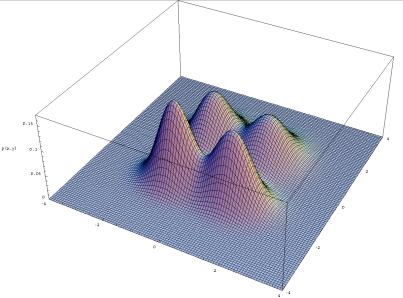
\includegraphics[width=0.7\linewidth]{Bimodal-bivariate-small.png}
\end{textblock*}

\end{frame}

\begin{frame}{混合分布}
\begin{itemize}
\item これまでは、全てのデータ$\bm{x}_1, \ldots, \bm{x}_N$が同じ分布から生成されると仮定していた
\item 一方、混合分布によるモデリングでは、同じ種類の分布だがパラメータの値が違う分布を$K$個用意する
\begin{itemize}
\item これらの分布をコンポーネントと呼ぶことがある
\end{itemize}
\item そして、各データ$\bm{x}_i$について…
\end{itemize}
\begin{enumerate}
\item カテゴリカル分布$\mbox{Cat}(\bm{\theta})$に従って
$K$個の分布から一つ選ぶ
\begin{itemize}
\item $\bm{\theta}=(\theta_1,\ldots,\theta_K)$は混合分布のパラメータ。
\item $\theta_k$は$k$番目の分布が選ばれる確率。$\sum_{k=1}^K \theta_k = 1$が成り立つ
\end{itemize}
\item そして、$\bm{x}_i$の値がその選ばれた分布に従うと考える。
\end{enumerate}
\end{frame}


\section{混合正規分布}

\begin{frame}\frametitle{Contents}
\Large \tableofcontents[currentsection]
\end{frame}

\begin{frame}{混合正規分布}
\begin{itemize}
\item 混合正規分布を使ったモデリングでは、
各$\bm{x}_i$が以下のように生成されると仮定する
\end{itemize}
\vspace{.1in}
\begin{enumerate}
\item カテゴリカル分布$\mbox{Cat}(\bm{\theta})$から、
確率変数$z_i$の値をdrawする
\begin{itemize}
\item 「$z_i = k$」は、$\bm{x}_i$については$k$番目のコンポーネントが選ばれた、ということを意味する
\end{itemize}
\item その$z_i$の値に対応する確率分布から、$\bm{x}_i$をdrawする
\begin{itemize}
\item $\bm{\mu}_k, \bm{\Sigma}_k$は$k$番目のコンポーネントである正規分布のパラメータ
\end{itemize}
\begin{align}
z_i & \sim \mbox{Cat}(\bm{\theta}) \notag \\
\bm{x}_i & \sim \mathcal{N}(\bm{\mu}_{z_i}, \bm{\Sigma}_{z_i})
\end{align}
\end{enumerate}
\end{frame}

\begin{frame}{単変量正規分布の混合分布の場合}
\begin{itemize}
\item $K$個のコンポーネントのなかから一つを選ぶ際に使われるカテゴリカル分布のパラメータは
$\bm{\theta} = (\theta_1,\ldots,\theta_K)$
\begin{itemize}
\item $\theta_k$は$k$番目のコンポーネントが選ばれる確率
\item $\sum_{k=1}^K \theta_k = 1$が成り立つ
\end{itemize}
\item $K$個の単変量正規分布をコンポーネントとして用意する
\item $k$番目の分布のパラメータは、平均$\mu_k$と標準偏差$\sigma_k$
\begin{itemize}
\item つまり、$k$番目のコンポーネントの確率密度関数は
\end{itemize}
\begin{align}
p(x;\mu_k,\sigma_k) = \frac{1}{\sqrt{2\pi\sigma_k^2}}\exp\Big( - \frac{(x - \mu_k)^2}{2\sigma_k^2} \Big)
\end{align}
\end{itemize}
\end{frame}

\begin{frame}{単変量正規分布の混合分布における同時分布}
\vspace{-.1in}
\begin{itemize}
\item 観測されたデータを表す確率変数$\mathcal{X} = \{x_1, \ldots, x_N\}$と、
\item[] コンポーネントへの所属を表す確率変数$\mathcal{Z} = \{z_1,\ldots,z_N\}$との同時分布は
\vspace{-.1in}
\begin{align}
& p( \mathcal{X}, \mathcal{Z} ;\bm{\theta}, \{ \mu_k \}, \{ \sigma_k \})
= \prod_{i=1}^N p(z_i ; \theta_{z_i}) p(x_i | z_i ; \mu_{z_i}, \sigma_{z_i})
\notag \\ &
= \prod_{i=1}^N \bigg[ \theta_{z_i} \times \frac{1}{\sqrt{2\pi\sigma_{z_i}^2}}\exp\bigg( - \frac{(x_i - \mu_{z_i})^2 }{2\sigma_{z_i}^2} \bigg) \bigg]
\label{eq:joint_MN}
\end{align}
\vspace{-.15in}
\begin{itemize}
\item $z_i$は$x_i$が属するコンポーネントを表す
\item $p(z_i)$はカテゴリカル分布$\mbox{Cat}(\bm{\theta})$のpmfから計算される$z_i$の尤度
\item $p(x_i | z_i)$は正規分布$\mathcal{N}(\mu_{z_i}, \sigma_{z_i})$のpdfから計算される$x_i$の尤度
\end{itemize}
\end{itemize}
\end{frame}


\section{混合正規分布:教師ありの場合}

\begin{frame}\frametitle{Contents}
\Large \tableofcontents[currentsection]
\end{frame}


\begin{frame}{教師ありの設定の場合 (1/2)}
\begin{itemize}
\item 教師ありの設定で、混合分布のパラメータを最尤推定する
\item 教師ありの設定の場合、各データ$x_i$について、それがどのコンポーネントから生成されたかは、すでに分かっている
\item 言い換えれば、$z_i$の値も観測データに含まれる
\begin{itemize}
\item つまり、観測データを$\mathcal{D}$で表すとすると、$\mathcal{D} = \{ (x_1,z_1), \ldots, (x_N,z_N) \}$
\item $x_i$も$z_i$も、すでに観測されており、よって、固定されている
\end{itemize}
\item このとき、式\eqref{eq:joint_MN}の同時分布が、そのまま、観測データ$\mathcal{D}$の尤度を表すことになる
\end{itemize}
\end{frame}

\begin{frame}{教師ありの設定の場合 (2/2)}
\begin{itemize}
\item そして、観測データ$\mathcal{D} = \{ (x_1,z_1), \ldots, (x_N,z_N) \}$の尤度は、下のように書き直すことができる
\vspace{-.1in}
\begin{align}
& p(\mathcal{D};\bm{\theta}, \{ \mu_k \}, \{ \sigma_k \} )
= \prod_{i=1}^N p(z_i ; \theta_{z_i}) p(x_i | z_i ; \mu_{z_i}, \sigma_{z_i})
\notag \\ &
= \prod_{i=1}^N \bigg[ \theta_{z_i} \times \frac{1}{\sqrt{2\pi\sigma_{z_i}^2}}\exp\bigg( - \frac{(x_i - \mu_{z_i})^2}{2\sigma_{z_i}^2} \bigg) \bigg]
\notag \\ &
= \prod_{k=1}^K \bigg[ \theta_k^{c_k} \times \frac{1}{ (\sqrt{2\pi\sigma_k^2} )^{c_k}} 
\exp\bigg( - \frac{ \sum_{ \{ i : z_i = k \} } (x_i - \mu_k)^2 }{2\sigma_k^2} \bigg) \bigg]
\label{eq:likelihood_MN}
\end{align}
\vspace{-.15in}
\begin{itemize}
\item $c_k$は、$k$番目のコンポーネントに属するデータの個数
\end{itemize}
\end{itemize}
\end{frame}


\begin{frame}{教師ありの場合の混合正規分布の最尤推定}
\begin{itemize}
\item 混合正規分布のパラメータを、式\eqref{eq:likelihood_MN}の観測データの尤度を最大化することによって推定する方法を、以下に示す
\end{itemize}
\end{frame}


\begin{frame}
\FontMath
\vspace{.1in}
目的関数を$L(\bm{\theta},\{ \mu_k \}, \{ \sigma_k \})$とおくと、
\begin{align}
& L(\bm{\theta},\{ \mu_k \}, \{ \sigma_k \})
= \ln p(\mathcal{D};\bm{\theta},\{ \mu_k \}, \{ \sigma_k \}) 
+ \lambda \bigg( 1 - \sum_{k=1}^K \theta_k \bigg)
\notag \\ &
= \sum_{k=1}^K c_k \ln \theta_k - \sum_{k=1}^K c_k \ln \sigma_k
- \sum_{k=1}^K \frac{\sum_{ \{ i : z_i = k \} } (x_i - \mu_k)^2}{ 2\sigma_k^2} + \lambda \bigg( 1 - \sum_{k=1}^K \theta_k \bigg) + const.
\end{align}
目的関数$L$を、各パラメータで偏微分する。
\begin{align}
\frac{\partial L}{\partial \mu_k} = \frac{ \sum_{ \{ i : z_i = k \} } (x_i - \mu_k) }{\sigma_k^2}
= \frac{ \sum_{ \{ i : z_i = k \} } x_i - c_k \mu_k }{\sigma_k^2}
\end{align}
$\frac{\partial L}{\partial \mu_k} = 0$より、$\mu_k = \frac{ \sum_{ \{ i : z_i = k \} } x_i }{ c_k } = \bar{x}_k$を得る。
\begin{align}
\frac{\partial L}{\partial \sigma_k} = - \frac{c_k}{\sigma_k} + \frac{\sum_{ \{ i : z_i = k \} } (x_i - \mu_k)^2}{ \sigma_k^3}
\end{align}
$\frac{\partial L}{\partial \sigma_k} = 0$より、
$\sigma_k^2 = \frac{\sum_{ \{ i : z_i = k \} } (x_i - \bar{x}_k)^2}{ c_k}$を得る。
\end{frame}

\begin{frame}
\FontMath
\begin{align}
\frac{\partial L}{\partial \theta_k} = \frac{c_k}{\theta_k} - \lambda \mbox{ , \ }
\frac{\partial L}{\partial \lambda} = 1 - \sum_{k=1}^K \theta_k
\end{align}
$\frac{\partial L}{\partial \theta_k} = 0$より、$\theta_k = \frac{c_k}{\lambda}$を得る。

$\frac{\partial L}{\partial \lambda} = 0$より、$1 - \sum_{k=1}^K \frac{c_k}{\lambda} = 0$を得る。

つまり、$\lambda = \sum_k c_k$が言えるので、$\theta_k = \frac{c_k}{\sum_k c_k}$を得る。

\

まとめると、
\begin{itemize}
\item $\theta_k$は、$k$番目のコンポーネントから生成されたデータの割合となる。
\item $\mu_k$と$\sigma_k$は、$k$番目のコンポーネントから生成されたデータだけの尤度をもとに最尤推定した値となる。
\end{itemize}
\end{frame}


\section{混合正規分布:教師なしの場合}

\begin{frame}\frametitle{Contents}
\Large \tableofcontents[currentsection]
\end{frame}


\begin{frame}{教師なしの設定の場合}
\vspace{-.05in}
\begin{itemize}
\item 教師なしの設定の場合、各データ$x_i$について、それがどのコンポーネントから生成されたかは、分からない!
\item すなわち、$z_i$は潜在変数latent variables
\begin{itemize}
\item つまり、$\mathcal{X} = \{ x_1, \ldots, x_N \}$だけが観測変数
\item 一方、潜在変数の集合を$\mathcal{Z} = \{ z_1, \ldots, z_N \}$とする
\end{itemize}
\item 観測変数と潜在変数の同時分布$p(\mathcal{X}, \mathcal{Z})$は、式\eqref{eq:joint_MN}と同じで
\vspace{-.13in}
\begin{align}
& p(\mathcal{X}, \mathcal{Z};\bm{\theta},\{ \mu_k \}, \{ \sigma_k \})
= \prod_{i=1}^N p(z_i ; \theta_{z_i}) p(x_i | z_i ; \mu_{z_i}, \sigma_{z_i})
\notag \\ &
= \prod_{i=1}^N \bigg[ \theta_{z_i} \times \frac{1}{\sqrt{2\pi\sigma_{z_i}^2}}\exp\bigg( - \frac{(x_i - \mu_{z_i})^2}{2\sigma_{z_i}^2} \bigg) \bigg]
\notag
\end{align}
\end{itemize}
\end{frame}

\begin{frame}{教師なしの場合の観測データの尤度}
\begin{itemize}
\item 潜在変数を含むモデリングの場合、観測データの尤度$p(\mathcal{X})$は、
潜在変数$\mathcal{Z}$を周辺化してはじめて得られる
\begin{itemize}
\item 潜在変数を周辺化する=潜在変数がとりうる値の全てを考慮する
\end{itemize}
\begin{align}
p(\mathcal{X}) & = \sum_{\mathcal{Z}} p(\mathcal{X}, \mathcal{Z})
= \sum_{z_1=1}^K \sum_{z_2=1}^K \cdots \sum_{z_{N-1}=1}^K \sum_{z_N=1}^K p(\mathcal{X}, \mathcal{Z})
\notag \\ &
= \sum_{z_1=1}^K \sum_{z_2=1}^K \cdots \sum_{z_{N-1}=1}^K \sum_{z_N=1}^K \prod_{i=1}^N p(x_i, z_i)
\notag \\ &
= \prod_{i=1}^N \bigg( \sum_{z_i=1}^K p(x_i , z_i) \bigg)
= \prod_{i=1}^N \bigg( \sum_{z_i=1}^K p(z_i) p(x_i | z_i) \bigg)
\label{eq:LH_mixture}
\end{align}
\end{itemize}
\end{frame}


\begin{frame}{教師なしの場合の観測データの対数尤度}
\begin{itemize}
\item よって、対数尤度は、式\eqref{eq:joint_MN}と式\eqref{eq:LH_mixture}より
\vspace{-.1in}
\begin{align}
& \ln p(\mathcal{X}) = \ln \sum_{\mathcal{Z}} p(\mathcal{X}, \mathcal{Z})
= \ln \prod_{i=1}^N \bigg( \sum_{z_i=1}^K p(x_i , z_i) \bigg)
\notag \\ &
= \ln \prod_{i=1}^N \bigg( \sum_{z_i=1}^K p(z_i) p(x_i | z_i) \bigg)
= \sum_{i=1}^N \ln \bigg( \sum_{z_i=1}^K p(z_i) p(x_i | z_i) \bigg)
\notag \\ &
= \sum_{i=1}^N \ln \bigg( \sum_{z_i=1}^K \bigg[ \theta_{z_i} \times \frac{1}{\sqrt{2\pi\sigma_{z_i}^2}}\exp\Big( - \frac{(x_i - \mu_{z_i})^2}{2\sigma_{z_i}^2} \Big) \bigg] \bigg)
\label{eq:logLH_MN}
\end{align}
\end{itemize}
\end{frame}

\begin{frame}{観測データの対数尤度の最大化?}
\begin{itemize}
\item あとは、対数尤度$\ln p(\mathcal{X}) = \sum_{i=1}^N \ln \Big( \sum_{z_i=1}^K p(z_i) p(x_i | z_i) \Big)$を最大にする$\bm{\theta}=(\theta_1,\ldots,\theta_K)$や$\mu_1,\ldots,\mu_K$や$\sigma_1,\ldots,\sigma_K$を求めれば良い・・・???
\begin{itemize}
\item 式\eqref{eq:logLH_MN}をそのまま最大化することはしない
\end{itemize}
\end{itemize}
\end{frame}


\begin{frame}{積の対数と和の対数}
\begin{itemize}
\item 何かを掛け算したものの対数は、何かの対数の和に書き直せるので、扱いやすい
\begin{align}
\log(a \times b) = \log(a) + \log(b)
\end{align}
\item 何かを足し算したものの対数は、それ以上変形のしようがないので、扱いにくい
\begin{align}
\log(a + b) = \ldots
\end{align}\end{itemize}
\end{frame}

\begin{frame}{イェンセンの不等式(対数関数の場合)}
\begin{itemize}
\item $p_1,\ldots,p_K$を、$\sum_{k=1}^K p_k=1$を満たす正の実数とする
\item また、$x_1,\ldots, x_K$を正の実数とする
\item このとき、以下の不等式が成り立つ
\begin{align}
\ln \bigg( \sum_{k=1}^K p_k x_k \bigg) \geq \sum_{k=1}^K p_k \ln(x_k)
\end{align}
\begin{itemize}
\item 和の対数(扱いにくい!)の下界lower boundを、
対数の和(扱いやすい!)として得るため、イェンセンの不等式をよく使う
\item なお、対数関数に限らず、上に凸な関数なら、上の不等式は成立
\end{itemize}
\end{itemize}
\end{frame}

\begin{frame}{観測データの対数尤度の下界}
\begin{itemize}
\item イェンセンの不等式を利用して$\ln p(\mathcal{X})$の下界を得たい
\item そこで、各$x_i$について$\bm{q}_i \equiv (q_{i,1}, \ldots, q_{i,K})$という$\sum_k q_{i,k}=1$を満たす変数を用意すると
\begin{align}
& \ln p(\mathcal{X}) = \sum_{i=1}^N \ln \Big( \sum_{z_i=1}^K p(z_i) p(x_i | z_i) \Big)
\notag \\ & = \sum_{i=1}^N \ln \Big( \sum_{z_i=1}^K q_{i,z_i} \frac{p(z_i) p(x_i | z_i)}{q_{i,z_i}} \Big)
\geq 
\sum_{i=1}^N \sum_{z_i=1}^K q_{i,z_i} \ln\frac{p(z_i) p(x_i | z_i)}{q_{i,z_i}}
\label{eq:LB}
\end{align}
\vspace{-.2in}
\item この下界を$\mathcal{L}(\{ \bm{q}_i \},\bm{\theta},\{\mu_k\},\{\sigma_k\})$と書くことにする
\end{itemize}
\end{frame}

\begin{frame}{観測データの対数尤度の下界の最大化}
\begin{itemize}
\item $\ln p(\mathcal{X})$の代わりに$\mathcal{L}(\{ \bm{q}_i \},\bm{\theta},\{\mu_k\},\{\sigma_k\})$を最大化することによって、次の未知量を推定する
\begin{itemize}
\item 新たに導入した$\{ \bm{q}_i \} \equiv \{ \bm{q}_1, \ldots, \bm{q}_N \}$ where $\bm{q}_i=(q_{i,1},\ldots,q_{i,K})$
\item モデルパラメータ$\bm{\Theta} \equiv \{ \bm{\theta}, \{ \mu_k \}, \{ \sigma_k \} \}$
\end{itemize}
\item いま考えている単変量正規分布の混合分布の場合
\begin{align}
p(z_i=k) & = \theta_k \\
p(x_i | z_i=k) & = \frac{1}{\sqrt{2\pi\sigma_k^2}} \exp \bigg( - \frac{ ( x_i - \mu_k)^2 }{ 2\sigma_k^2 } \bigg)
\end{align}
\item これらを式\eqref{eq:LB}に当てはめることで、以下、推定計算を行う
\end{itemize}
\end{frame}

\begin{frame}
\FontMath
\begin{align}
& L(\{ \bm{q}_i \},\bm{\theta},\{\mu_k\},\{\sigma_k\}) 
\notag \\ &
= \mathcal{L}(\{ \bm{q}_i \},\bm{\theta},\{\mu_k\},\{\sigma_k\})
+ \sum_{i=1}^N \lambda_i \bigg(1 - \sum_{k=1}^K q_{i,k}\bigg)
+ \lambda_0 \bigg( 1 - \sum_{k=1}^K \theta_k \bigg)
\notag \\ &
= \sum_{i=1}^N \sum_{k=1}^K q_{i,k} \ln\frac{\theta_k p(x_i | z_i = k)}{q_{i,k}}
+ \sum_{i=1}^N \lambda_i \bigg(1 - \sum_{k=1}^K q_{i,k}\bigg)
+ \lambda_0 \bigg( 1 - \sum_{k=1}^K \theta_k \bigg)
\notag \\ &
= 
\sum_{i=1}^N \sum_{k=1}^K q_{i,k} \ln \big( \theta_k p(x_i | z_i = k) \big)
- \sum_{i=1}^N \sum_{k=1}^K q_{i,k} \ln q_{i,k}
+ \sum_{i=1}^N \lambda_i \bigg(1 - \sum_{k=1}^K q_{i,k}\bigg)
+ \lambda_0 \bigg( 1 - \sum_{k=1}^K \theta_k \bigg)
\end{align}
\begin{align}
\frac{\partial L}{\partial q_{i,k}}
= \ln \big( \theta_k p(x_i | z_i = k) \big) - \ln q_{i,k} - 1 - \lambda_i
\end{align}
$\frac{\partial L}{\partial q_{i,k}}$ = 0と$\sum_k q_{i,k}=1$より
$q_{i,k} = \frac{ \theta_k p(x_i | z_i = k) }{ \sum_k \theta_k p(x_i | z_i = k) }$を得る。
\end{frame}

\begin{frame}
\FontMath
$q_{i,k} \ln \big( \theta_k p(x_i | z_i = k) \big)
= q_{i,k} \ln \theta_k + q_{i,k} \ln p(x_i | z_i = k)$より、
\begin{align}
\frac{\partial L}{\partial \theta_k}
= \frac{ \sum_{i=1}^N  q_{i,k} }{ \theta_k } - \lambda_0
\end{align}
$\frac{\partial L}{\partial \theta_k} = 0$と$\sum_k \theta_k = 1$より
$\theta_k = \frac{ \sum_{i=1}^N q_{i,k} }{ \sum_{k=1}^K \sum_{i=1}^N q_{i,k} } = \frac{ \sum_{i=1}^N q_{i,k} }{ N }$を得る。

\

$\frac{\partial }{\partial \mu_k} \ln p(x_i | z_i = k) = \frac{ x_i - \mu_k }{\sigma_k^2}$と
$\frac{\partial }{\partial \sigma_k} \ln p(x_i | z_i = k) = - \frac{1}{\sigma_k} + \frac{ (x_i - \mu_k)^2 }{\sigma_k^3}$より
\begin{align}
\frac{\partial L}{\partial \mu_k}
& = \frac{ \sum_{i=1}^N q_{i,k} (x_i - \mu_k) }{\sigma_k^2} \\
\frac{\partial L}{\partial \sigma_k}
& = \frac{ \sum_{i=1}^N q_{i,k} ( - \sigma_k^2 + (x_i - \mu_k)^2 ) }{\sigma_k^3}
\end{align}
$\frac{\partial L}{\partial \mu_k} = 0$より
$\mu_k = \frac{ \sum_{i=1}^N q_{i,k} x_i }{ \sum_{i=1}^N q_{i,k} }$を得る。
また、$\frac{\partial L}{\partial \sigma_k} = 0$より
$\sigma_k^2 = \frac{ \sum_{i=1}^N q_{i,k} (x_i - \mu_k)^2 }{ \sum_{i=1}^N q_{i,k} }$を得る。
\end{frame}

\begin{frame}{混合正規分布のためのEMアルゴリズム}
\vspace{-.1in}
\begin{itemize}
\item E step
\vspace{-.1in}
\begin{align}
q_{i,k} \leftarrow \frac{ \theta_k p(x_i | z_i = k) }{ \sum_k \theta_k p(x_i | z_i = k) }
\label{eq:EM_q}
\end{align}
\vspace{-.1in}
\begin{itemize}
\item[] ただし$p(x_i | z_i = k) = \frac{1}{\sqrt{2\pi\sigma_k^2}} \exp\big( - \frac{ (x_i - \mu_k)^2 }{2\sigma_k^2} \big)$
\end{itemize}
\vspace{-.1in}
\item M step
\vspace{-.1in}
\begin{align}
\theta_k & \leftarrow \frac{ \sum_{i=1}^N q_{i,k} }{ N } \\
\mu_k & \leftarrow \frac{ \sum_{i=1}^N q_{i,k} x_i }{ \sum_{i=1}^N q_{i,k} } \\
\sigma_k^2 & \leftarrow \frac{ \sum_{i=1}^N q_{i,k} (x_i - \mu_k)^2 }{ \sum_{i=1}^N q_{i,k} }
\end{align}
\end{itemize}
\end{frame}

\begin{frame}{$q_{i,k}$とは何なのか(1/4)}
\begin{itemize}
\item イェンセンの不等式を使って、次の下界を得たのだった
\begin{align}
\sum_{i=1}^N \ln \Big( \sum_{z_i=1}^K p(z_i) p(x_i | z_i) \Big)
\geq 
\sum_{i=1}^N \sum_{z_i=1}^K q_{i,z_i} \ln\frac{p(z_i) p(x_i | z_i)}{q_{i,z_i}}
\notag
\end{align}
\item 左辺から右辺を引くと
\end{itemize}
\begin{align}
& \sum_{i=1}^N \ln \Big( \sum_{z_i=1}^K p(z_i) p(x_i | z_i) \Big)
- \sum_{i=1}^N \sum_{z_i=1}^K q_{i,z_i} \ln\frac{p(z_i) p(x_i | z_i)}{q_{i,z_i}}
\notag \\ &
= \sum_{i=1}^N \sum_{z_i=1}^K q_{i,z_i} \ln \Big( \sum_{z_i=1}^K p(z_i) p(x_i | z_i) \Big)
- \sum_{i=1}^N \sum_{z_i=1}^K q_{i,z_i} \ln\frac{p(z_i) p(x_i | z_i)}{q_{i,z_i}}
\notag
\end{align}
\end{frame}

\begin{frame}{$q_{i,k}$とは何なのか(2/4)}
(続き)
\begin{align}
&
= \sum_{i=1}^N \sum_{z_i=1}^K q_{i,z_i} \ln \Big( \sum_{z_i=1}^K p(x_i, z_i) \Big)
- \sum_{i=1}^N \sum_{z_i=1}^K q_{i,z_i} \ln\frac{p(z_i) p(x_i | z_i)}{q_{i,z_i}}
\notag \\
& = \sum_{i=1}^N \sum_{z_i=1}^K q_{i,z_i} \ln p(x_i)
- \sum_{i=1}^N \sum_{z_i=1}^K q_{i,z_i} \ln\frac{p(x_i, z_i)}{q_{i,z_i}}
\notag \\& 
= \sum_{i=1}^N \sum_{z_i=1}^K q_{i,z_i} \ln \frac{p(x_i) q_{i,k}}{p(x_i , z_i)}
= \sum_{i=1}^N \sum_{z_i=1}^K q_{i,z_i} \ln \frac{q_{i,z_i}}{p(z_i | x_i)}
\label{eq:diff}
\end{align}
\begin{itemize}
\item $q_{i,k}=p(z_i = k| x_i)$のとき、等号が成立する
\end{itemize}
\end{frame}


\begin{frame}{カルバック・ライブラー情報量}
\begin{itemize}
\item $p,q$を離散確率分布とすると、
$q$から$p$への{\small($p$の$q$に対する)}
カルバック・ライブラー情報量 {\small Kullback\UTF{2013}Leibler divergence}とは
\begin{align}
\infdiv{p}{q} = \sum_{x} p(x) \ln \frac{p(x)}{q(x)}
\end{align}
\item $p,q$が連続確率分布の場合は
\begin{align}
\infdiv{p}{q} = \int p(x) \ln \bigg( \frac{p(x)}{q(x)} \bigg) dx
\end{align}
\item $p=q$ならば、またそのときに限り$\infdiv{p}{q} = 0$
\item[注.] $q(x) = 0$なのに$p(x) \neq 0$となる$x$があってはいけない!
\end{itemize}
\end{frame}

\begin{frame}{$q_{i,k}$とは何なのか(3/4)}
\vspace{-.05in}
\begin{itemize}
\item $q_i(z_i)$を、$K$個のアイテム$\{1,\ldots,K\}$上に定義されたカテゴリカル分布とし、
$q_i(z_i=k) \equiv q_{i,k}$と設定する
\item 式\eqref{eq:diff}は$q_i(z_i)$の$p(z_i|x_i)$に対するカルバック・ライブラー情報量になっている
\item ところで、式\eqref{eq:EM_q}より、
\begin{align}
q_{i,k} & = \frac{ \theta_k p(x_i | z_i = k) }{ \sum_k \theta_k p(x_i | z_i = k) }
= \frac{p(z_i=k)p(x_i|z_i=k)}{\sum_k p(z_i=k)p(x_i|z_i=k)}
\notag \\ &
= \frac{p(x_i,z_i=k)}{\sum_k p(x_i,z_i=k)} = \frac{p(x_i,z_i=k)}{p(x_i)} = p(z_i=k|x_i)
\end{align}
\end{itemize}
\end{frame}

\begin{frame}{$q_{i,k}$とは何なのか(4/4)}
\begin{itemize}
\item つまり、式\eqref{eq:EM_q}は$q_{i,k} = p(z_i=k|x_i)$を意味している
\item このとき、式\eqref{eq:diff}のカルバック・ライブラー情報量は\underline{ゼロ}!
\item ただし、$q_{i,k}$は、モデルパラメータ$\bm{\theta},\{\mu_k\},\{\sigma_k\}$の値を固定し、
$\ln p(x_i)$の下界を最大化することで求めたものである
\begin{itemize}
\item つまり、モデルパラメータの特定の値について式\eqref{eq:diff}をゼロにできるだけで、
$\ln p(x_i)$が最大化できているわけではないが…
\end{itemize}
\item Eステップでは、その固定されたパラメータ値に対しては、各$q_{i,k}$について最善の答えを得ていることは確か
\item Mステップでは、$\{ \bm{q}_i \}$の値を固定し、$\ln p(x_i)$の下界をできるだけ大きくすべく、
パラメータの値を求めている
\end{itemize}
\end{frame}


\begin{frame}{E stepで何をしているか}
\begin{itemize}
\item モデルのパラメータ$\bm{\Theta} \equiv \{ \bm{\theta}, \mu_1, \ldots, \mu_K, \sigma_1, \ldots, \sigma_K \}$の値を固定した状態で、
対数尤度の下界$\mathcal{L}(\bm{\Theta})$を最大化する$\{ \bm{q}_i \}$を求めているのが、E step
\item パラメータ$\bm{\Theta}$の、固定された値を、$\bm{\Theta}_{\mbox{\scriptsize old}}$と書くことにする
\item その最大化によって得られる答えは
\begin{align}
q_{i, k} = p(z_i = k|x_i; \bm{\Theta}_{\mbox{\scriptsize old}})
\end{align}
\item つまり、モデルパラメータ$\bm{\Theta}$の値を固定したうえで、観測データを所与とする潜在変数の条件付き分布を求めている
\end{itemize}
\end{frame}


\section{混合多項分布:教師なしの場合}

\begin{frame}\frametitle{Contents}
\Large \tableofcontents[currentsection]
\end{frame}


\begin{frame}{多項分布の混合分布}
\begin{itemize}
\item 第$k$コンポーネントのパラメータを$\bm{\phi}_k$とする
\begin{itemize}
\item $\bm{\phi}_k = (\phi_{k,1},\ldots,\phi_{k,W})$
\item $\phi_{k,w}$は第$k$コンポーネントに属する文書での単語$\mbox{v}_w$の出現確率
\end{itemize}
\item $\ln p(\mathcal{X})$の代わりに$\mathcal{L}(\{q_{i,k}\},\bm{\theta}, \{ \bm{\phi}_k \})$を最大化
\item 多項分布の混合分布の場合
\begin{align}
p(z_i=k) & = \theta_k \\
p(\mathcal{D}_i | z_i=k) & = \frac{n_i!}{\prod_w c_{i,w}!} \prod_{w=1}^W \phi_{k,w}^{c_{i,w}}
\end{align}
\item 以下、推定計算を行う
\end{itemize}
\end{frame}

\begin{frame}
\FontMath
\begin{align}
& L(\{q_{i,k}\},\bm{\theta}, \{ \bm{\phi}_k \} ) 
\notag \\ &
= \mathcal{L}(\{q_{i,k}\},\bm{\theta},\{ \bm{\phi}_k \})
+ \sum_{i=1}^N \lambda_i \bigg(1 - \sum_{k=1}^K q_{i,k}\bigg)
+ \lambda_0 \bigg( 1 - \sum_{k=1}^K \theta_k \bigg)
+ \sum_{k=1}^K \nu_k \bigg( 1 - \sum_{w=1}^W \phi_{k,w} \bigg)
\notag \\ &
= \sum_{i=1}^N \sum_{k=1}^K q_{i,k} \ln\frac{\theta_k p(\mathcal{D}_i | z_i = k)}{q_{i,k}}
+ \sum_{i=1}^N \lambda_i \bigg(1 - \sum_{k=1}^K q_{i,k}\bigg)
+ \lambda_0 \bigg( 1 - \sum_{k=1}^K \theta_k \bigg)
+ \sum_{k=1}^K \nu_k \bigg( 1 - \sum_{w=1}^W \phi_{k,w} \bigg)
\notag \\ &
= 
\sum_{i=1}^N \sum_{k=1}^K q_{i,k} \ln \big( \theta_k p(\mathcal{D}_i | z_i = k) \big)
- \sum_{i=1}^N \sum_{k=1}^K q_{i,k} \ln q_{i,k}
\notag \\ & \mbox{ \ \ }
+ \sum_{i=1}^N \lambda_i \bigg(1 - \sum_{k=1}^K q_{i,k}\bigg)
+ \lambda_0 \bigg( 1 - \sum_{k=1}^K \theta_k \bigg)
+ \sum_{k=1}^K \nu_k \bigg( 1 - \sum_{w=1}^W \phi_{k,w} \bigg)
\end{align}
\begin{align}
\frac{\partial L}{\partial q_{i,k}}
= \ln \big( \theta_k p(\mathcal{D}_i | z_i = k) \big) - \ln q_{i,k} - 1 - \lambda_i
\end{align}
$\frac{\partial L}{\partial q_{i,k}}$ = 0と$\sum_k q_{i,k}=1$より
$q_{i,k} = \frac{ \theta_k p(\mathcal{D}_i | z_i = k) }{ \sum_k \theta_k p(\mathcal{D}_i | z_i = k) }$を得る。
\end{frame}

\begin{frame}
\FontMath
$q_{i,k} \ln \big( \theta_k p(\mathcal{D}_i | z_i = k) \big)
= q_{i,k} \ln \theta_k + q_{i,k} \ln p(\mathcal{D}_i | z_i = k)$より、
\begin{align}
\frac{\partial L}{\partial \theta_k}
= \frac{ \sum_{i=1}^N  q_{i,k} }{ \theta_k } - \lambda_0
\end{align}
$\frac{\partial L}{\partial \theta_k} = 0$と$\sum_k \theta_k = 1$より
$\theta_k = \frac{ \sum_{i=1}^N q_{i,k} }{ \sum_{k=1}^K \sum_{i=1}^N q_{i,k} } = \frac{ \sum_{i=1}^N q_{i,k} }{ N }$を得る。

\

$\frac{\partial }{\partial \phi_{k,w}} \ln p(\mathcal{D}_i | z_i = k) = \frac{ c_{i,w} }{ \phi_{k,w} }$より
\begin{align}
\frac{\partial L}{\partial \phi_{k,w}}
& = \frac{ \sum_{i=1}^N q_{i,k} c_{i,w} }{ \phi_{k,w} } - \nu_k
\end{align}
$\frac{\partial L}{\partial \phi_{k,w}} = 0$より
$\phi_{k,w} = \frac{ \sum_{i=1}^N q_{i,k} c_{i,w} }{ \sum_{w=1}^W \sum_{i=1}^N q_{i,k} c_{i,w} }$を得る。
\end{frame}

\begin{frame}{混合多項分布のためのEMアルゴリズム}
\vspace{-.1in}
\begin{itemize}
\item E step
\vspace{-.1in}
\begin{align}
q_{i,k} \leftarrow \frac{ \theta_k p(x_i | z_i = k) }{ \sum_k \theta_k p(x_i | z_i = k) }
\end{align}
\vspace{-.1in}
\begin{itemize}
\item[] ただし$p(x_i | z_i = k) = \frac{n_i!}{\prod_w c_{i,w}!} \prod_{w=1}^W \phi_{k,w}^{c_{i,w}}$、つまり
\begin{align}
q_{i,k} \leftarrow \frac{ \theta_k \prod_w \phi_{k,w}^{c_{i,w}} }{ \sum_k \theta_k \prod_w \phi_{k,w}^{c_{i,w}} } \notag
\end{align}
\end{itemize}
\vspace{-.1in}
\item M step
\vspace{-.1in}
\begin{align}
\theta_k & \leftarrow \frac{ \sum_{i=1}^N q_{i,k} }{ N } \\
\phi_{k,w} & \leftarrow \frac{ \sum_{i=1}^N q_{i,k} c_{i,w} }{ \sum_{w=1}^W \sum_{i=1}^N q_{i,k} c_{i,w} }
\end{align}
\end{itemize}
\end{frame}

\end{document}